\documentclass[11pt]{article}
\usepackage{booktabs}
\usepackage{natbib}
\usepackage{fullpage}
\usepackage{fancyhdr}

\usepackage{amsmath}
\usepackage{amssymb}
\usepackage{url}

\usepackage{listings}
\usepackage{color}
\lstset{%
        basicstyle=\footnotesize\ttfamily,
        showspaces=false,
        showstringspaces=false,
        tabsize=2,
        breaklines=false,
        breakatwhitespace=true,
        identifierstyle=\ttfamily,
        keywordstyle=\color[rgb]{0,0,1},
        commentstyle=\color[rgb]{0.133,0.545,0.133},
        stringstyle=\color[rgb]{0.627,0.126,0.941},
    }

\usepackage{graphicx}
\usepackage{qtree}

% header
\fancyhead{}
\fancyfoot{}
\fancyfoot[C]{\thepage}
\fancyhead[R]{Daniel Foreman-Mackey}
\fancyhead[L]{Statistical Natural Language Processing --- Homework 5}
\pagestyle{fancy}
\setlength{\headsep}{10pt}
\setlength{\headheight}{20pt}

% shortcuts
\newcommand{\Eq}[1]{Equation (\ref{eq:#1})}
\newcommand{\eq}[1]{Equation (\ref{eq:#1})}
\newcommand{\eqlabel}[1]{\label{eq:#1}}
\newcommand{\Fig}[1]{Figure~\ref{fig:#1}}
\newcommand{\fig}[1]{Figure~\ref{fig:#1}}
\newcommand{\figlabel}[1]{\label{fig:#1}}

\newcommand{\etal}{\emph{et al.}}

\newcommand{\pr}[1]{\ensuremath{p\left (#1 \right )}}
\newcommand{\lk}[1]{\ensuremath{\mathcal{L} \left ( #1 \right )}}
\newcommand{\bvec}[1]{\ensuremath{\boldsymbol{#1}}}
\newcommand{\dd}{\ensuremath{\, \mathrm{d}}}
\newcommand{\normal}[2]{\ensuremath{\mathcal{N} \left ( #1; #2 \right ) }}
\newcommand{\T}{^\mathrm{T}}

\newcommand{\data}{\mathcal{D}}
\newcommand{\code}[1]{{\sffamily #1}}
\DeclareMathOperator*{\argmax}{arg\,max}


\begin{document}

For this assignment, I leaded the data and extracted the probabilistic grammar
using Python and then implemented my CKY algorithm in C (because I couldn't
come up with a way of doing it without loops).
I used the NLTK\footnote{\url{http://nltk.org}} module for I/O because it
includes methods for reading Penn Treebank-style tagged trees.
I implemented the rest of the code by hand.
The training step of my algorithm is quite slow but my final inference
algorithm can parse a 20 word sentence in approximately one second.
All of the code that I used for this assignment and the source code for this
document is available on GitHub at \url{https://github.com/dfm/nlp} in the
\code{hw5} directory.

\section{Introduction}

In this assignment, I'm are solving the syntactic parsing problem.
Given a sentence, I would like to infer the syntactic tree structure with
maximum probability under an empirical probabilistic context-free grammar.
The grammar consists of lexical rules and non-terminal emission rules.
The lexical rules have the form
\begin{eqnarray}
p(\mathrm{POS} \to \mathrm{word}) &=& p(\mathrm{word}\,|\,\mathrm{POS})
\end{eqnarray}
where \code{POS} is a part-of-speech tag and \code{word} is a word (that may
or may not be in the known vocabulary).
I estimated these probabilities from the training data using the same method
as the provided Java framework.
The non-lexical rules can be unaries or binaries estimated as
\begin{eqnarray}
p(\mathrm{A} \to \mathrm{B}) &=& p(\mathrm{B}\,|\,\mathrm{A}) \\
                             &=& \frac{f(\mathrm{A}\to\mathrm{B})}
                                 {\sum_\mathrm{X} f(\mathrm{A}\to\mathrm{X})}
\end{eqnarray}
or
\begin{eqnarray}
p(\mathrm{A} \to \mathrm{B\,C}) &=& p(\mathrm{B},\,\mathrm{C}\,|\,\mathrm{A}) \\
                                &=& \frac{f(\mathrm{A}\to\mathrm{B\,C})}
                                    {\sum_\mathrm{X} f(\mathrm{A}\to\mathrm{X})}
\end{eqnarray}
respectively, where the sum over X includes both unary and binary emissions.

\section{Tree normalization}

Since the model that I'm using only includes unary and binary rules, we need
to normalize the training trees before building the grammar.
The standard normalization form is ``Chomsky normal form'' and the
normalization algorithm is defined by a few simple rules and choices.
In particular, an approximate normalization is normally a better choice than
the exact form because the grammar will generalize more robustly.
It is easiest to describe this algorithm by showning an example.
Tree~\ref{eq:normalization}a below shows a hypothetical tagged syntactic tree
with more general rules than just unaries and binaries.
A possible lossless---or infinite-order---normalization is shown in
tree~\ref{eq:normalization}b.
In this representation, the node subscripts indicate the names of the sibling
nodes in the original tree and the superscripts keep track of the parents of
the normalized clique.
The default baseline normalization given in the homework is an infinite
horizontal and zeroth order vertical Markovization.
The representation of this tree in that form is given in
tree~\ref{eq:normalization}c.
A lossier but potentially more general tree is shown in
tree~\ref{eq:normalization}d.
Specifically, this last normalization a first-order vertical and
first-order horizontal Markov process.
\begin{eqnarray}\eqlabel{normalization}
&\begin{array}{cc}
\mbox{(a) reference tree} &
\mbox{(b) lossless normalization} \\
\hspace{0.3in}
\Tree [.S [.A [.B ] [.C ] [.D ] [.E ]]]
\hspace{0.3in} & \hspace{0.3in}
\Tree [.S [.A^S [.B ] [.A^S_{C,D,E} [.C ] [.A^S_{D,E} [.D ] [.E ]]]]]
\hspace{0.3in}
\end{array}& \nonumber\\
&\begin{array}{cc}
\mbox{(c) baseline normalization} &
\mbox{(d) finite-order Markovization} \\
\hspace{0.3in}
\Tree [.S [.A [.B ] [.A_{C,D,E} [.C ] [.A_{D,E} [.D ] [.E ]]]]]
\hspace{0.3in} & \hspace{0.3in}
\Tree [.S [.A^S [.B ] [.A^S_{C} [.C ] [.A^S_{D} [.D ] [.E ]]]]]
\hspace{0.3in}
\end{array}&
\end{eqnarray}

\section{Inference of tree structure}

The inference problem that we need to solve for this assignment is
\begin{eqnarray}
    G^* &=& \argmax_{G} p (G\,|\,\bvec{w})
\end{eqnarray}
where $G$ is the graph structure of the parse tree.
This probability can be factorized---assuming a local probabilistic
context-free grammar as discussed above---and evaluated for any given model.
The evaluation of the MAP graph is best performed using the CKY algorithm.
It took me a while to be able to wrap my head around the dynamic algorithm for
solving this problem---even though it is embarrassingly simple---and the
Youtube video posted by a
classmate\footnote{\url{https://www.youtube.com/watch?v=MiEKnFyErbQ}} was an
extremely useful resource.

After implementing a functional version of the algorithm (in pure Python), I
tried several different data structures in order to build an inference
algorithm that could solve a sentence in a bearable amount of time.
To do this, I was working directly in C with all of the tag names mapped to
integers.
In the end, the layout that I settled on was:
\begin{itemize}
\item{a flat list of unary rules,}
\item{a flat list of binary rules, and}
\item{sparse triangular representations of the node scores
      (log-probabilities) and back pointers.}
\end{itemize}
In my tests, this structure was more efficient than something more
sophisticated with support for child-major lookups but that might just be a
shortcoming of my experience with efficient data structures.
My final model---experiment F below---was able to parse a 20 word sentence in
about a second but I didn't do any real benchmark so there are probably some
other places to speed things up.

I also experimented with pruning to speed up the inference.
For simplicity, the prescription that I used was to discard any proposed
parents $N$ in a single span $C$ with scores
\begin{eqnarray}
    \log p_N &<& \max_C\,\log p - \theta
\end{eqnarray}
where $\theta$ is a free parameter and the maximization finds the highest
score in the clique.
While this technique does significantly reduce run time, I found that it had a
substantial negative impact on my results on the validation data so for all of
my experiments discussed here, I will set $\theta \ge 1000$ (the results seem
to be insensitive to the value when it is this large).

In practice, some sentences in the training data are not valid members of the
grammar---there is no path with finite probability from the \code{TOP} tag to
the observed sentence.
In these cases, I simply generated a dummy parse that emits the maximum
likelihood parts-of-speech from a \code{S} tag.
These sentences are quite rare but in a production system, it would probably
be a good idea to spend some time to build heuristic rules for corner cases
like this.

\section{Experiments}

Since the implementation of this inference algorithm took such a long time, I
only ran six production experiments for this assignment.
Each experiment was trained on all the training trees from the Penn Treebank
and validated on the sentences from the in-domain and out-of-domain
sentences with fewer than 41 words.
The differences between the experiments were only the orders of the
horizontal and vertical Markov processes.
I used the full CKY algorithm for each experiment so the exact maximum
probability tree should be recovered in each case.
This means that the only practical difference between experiments is the model
complexity and it would be a good idea to set the Markovization orders using
cross-validation on the development treebanks.
The runtime of the inference only scales linearly with the number of rules so
more complex models are still computationally tractable but they don't
necessarily generalize robustly due to sparsity in the training data.

The specification and F1 scores for each experiment are listed in
Table~\ref{tab:results}.
The F1 scores for the in-domain and out-of-domain validation sets are shown in
Figures~\ref{fig:in-domain} and~\ref{fig:out-of-domain} respectively.
In practice, I found that the performance on the test sentences (as evaluated
by the leader board) was significantly better (by $\sim 5\%$) than the
out-of-domain validation set.
As the model complexity increases most of the results improve but the most
complex model (F) doesn't generalize on the in-domain trees as well as model
E.
I found the same result when models E and F were compared on the test set.

\begin{table}[htbp]
\begin{center}
\begin{tabular}{ccccc}
\toprule
&\multicolumn{2}{c}{Markovization order}
&\multicolumn{2}{c}{F1 score [\%]} \\
experiment & horizontal & vertical & out-of-domain & in-domain \\\midrule
    A & $\infty$ & 0 & 57.137 & 65.674 \\
    B & 1 & 0 & 56.679 & 64.428 \\
    C & 2 & 0 & 58.146 & 65.413 \\
    D & 2 & 1 & 63.507 & 71.493 \\
    E & 2 & 2 & 63.945 & 73.050 \\
    F & 3 & 2 & 64.403 & 72.983 \\
\bottomrule
\end{tabular}
\end{center}
\caption{%
The specifications of the experiments and the resulting F1 scores.
\label{tab:results}}
\end{table}

\begin{figure}[htbp]
\begin{center}
    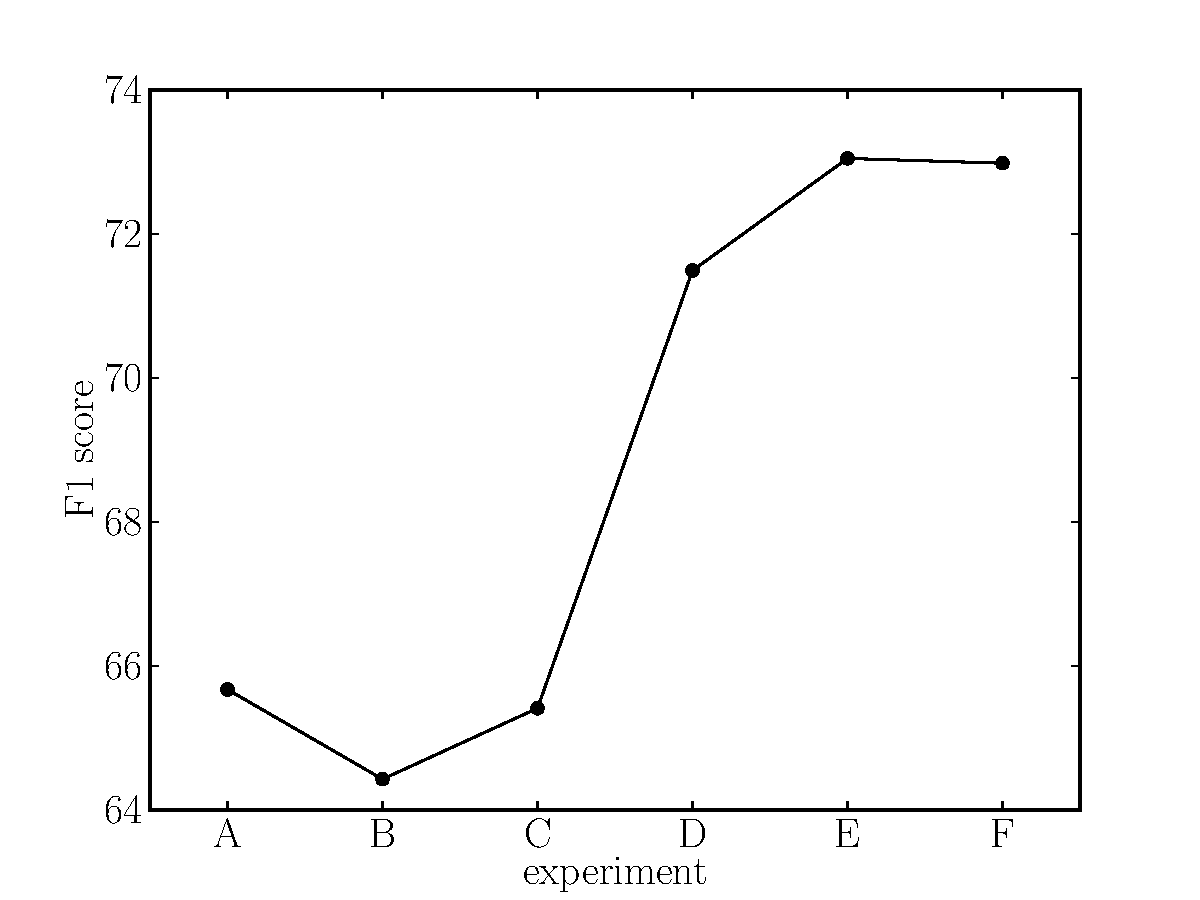
\includegraphics[width=0.7\textwidth]{in-domain.pdf}
\end{center}
\caption{%
The performance of the models on the in-domain validation trees.
This figure is sorted (roughly) by model complexity.
\figlabel{in-domain}}
\end{figure}

\begin{figure}[htbp]
\begin{center}
    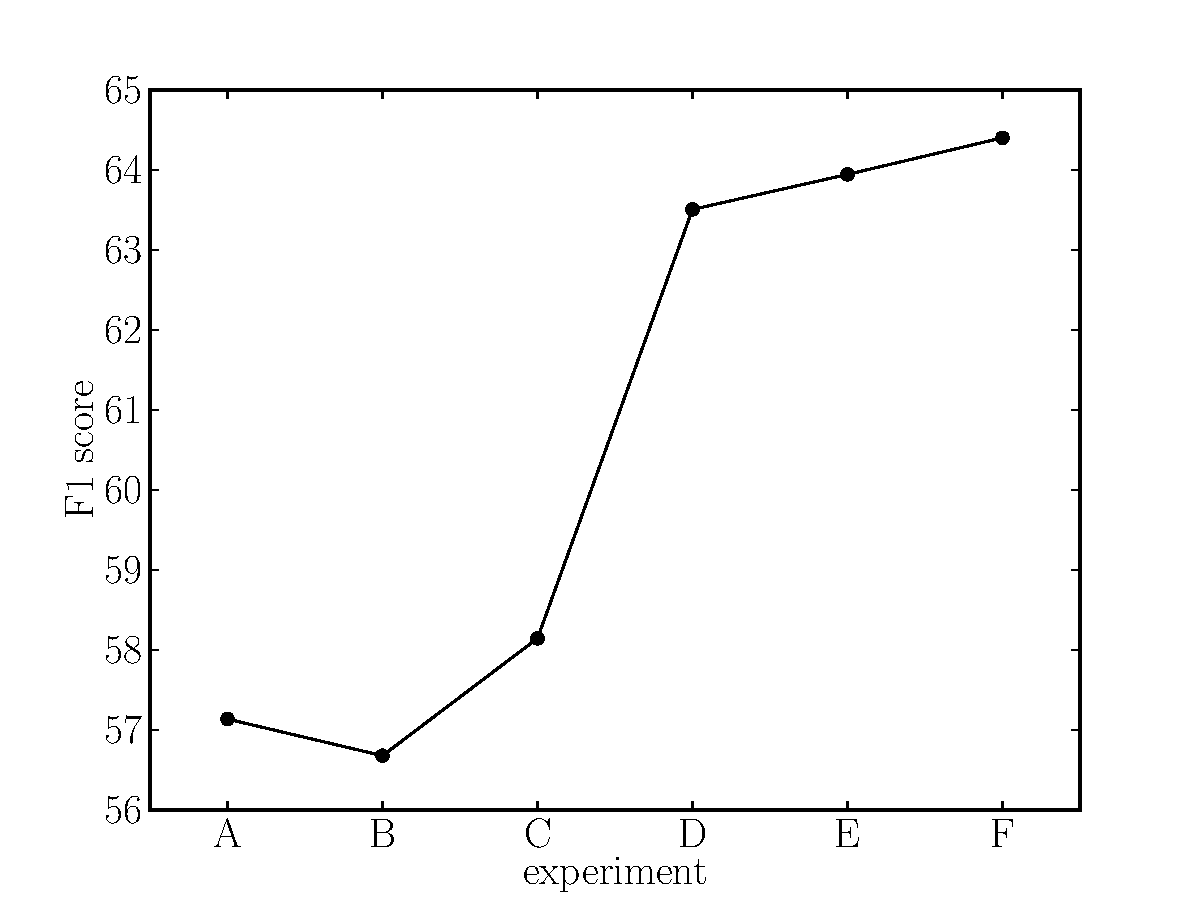
\includegraphics[width=0.7\textwidth]{out-of-domain.pdf}
\end{center}
\caption{%
The same as \fig{in-domain} for the out-of-domain validation set.
\figlabel{out-of-domain}}
\end{figure}

\end{document}
